\section{实验结果}
\subsection{实验数据介绍}


本部分实验数据分为两部分,一部分为Berkeley图像数据库BSDS500,另一部分为真实无人机航拍图像。使用Berkeley图像数据库主要是为了对比基于单像素和基于超像素两种最优分割算法的分割结果,并且在Berkeley图像数据库中自然景物图像中,目标物体一般只有一个,便于定性评估最优分割算法。使用无人机航拍图像主要是为了评估算法在复杂场景中的表现。

\begin{figure}[H]
\centering
    \subfigure[BSDS12003]
    {
        \label{Fig.sub.1}
        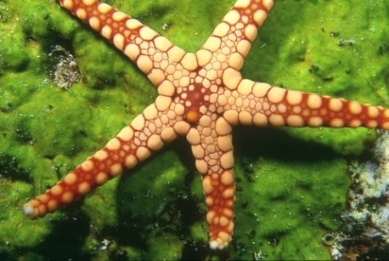
\includegraphics[width=2.4cm]{figures/BSDS12003.jpg}
    }
    \subfigure[BSDS118035]
    {
        \label{Fig.sub.1}
        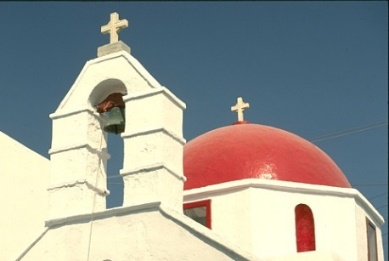
\includegraphics[width=2.4cm]{figures/BSDS118035.jpg}
    }
    \subfigure[BSDS8068]
    {
        \label{Fig.sub.1}
        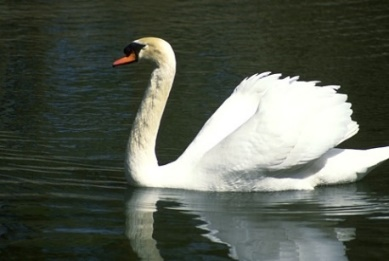
\includegraphics[width=2.4cm]{figures/BSDS8068.jpg}
    }
    \captionsetup{justification=centering}
    \caption{Berkeley 图像数据库 BSDS500 中的三张图像 \\ Fig.\ref{Berkeley图像数据库BSDS500中的三张图像} Three of the Berkeley Image Database BSDS500 Images}\label{Berkeley图像数据库BSDS500中的三张图像}
\end{figure}



\begin{figure}[H]
\centering
    \subfigure[航拍图像1]
    {
        \label{Fig.sub.1}
        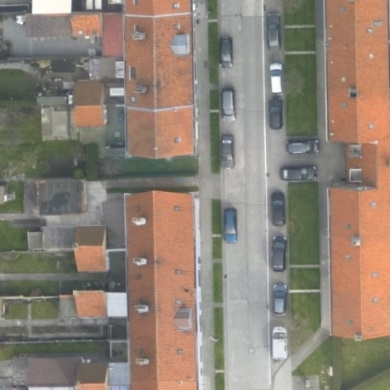
\includegraphics[width=2.4cm]{figures/无人机航拍图像1.jpg}
    }
    \subfigure[航拍图像2]
    {
        \label{Fig.sub.1}
        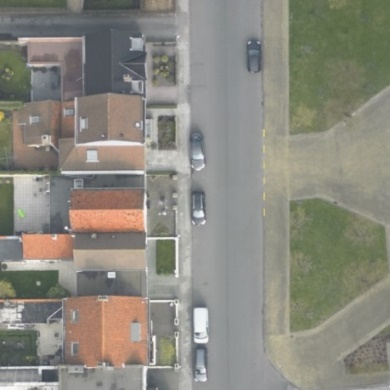
\includegraphics[width=2.4cm]{figures/无人机航拍图像2.jpg}
    }
    \subfigure[航拍图像3]
    {
        \label{Fig.sub.1}
        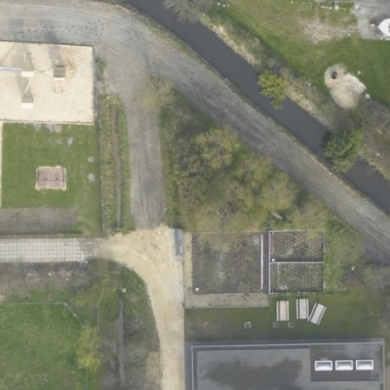
\includegraphics[width=2.4cm]{figures/无人机航拍图像3.jpg}
    }
    \captionsetup{justification=centering}
    \caption{三张无人机航拍图像 \\ Fig.\ref{三张无人机航拍图像} Three Unmanned Aerial Images}\label{三张无人机航拍图像}
\end{figure}





\subsection{基于单像素的最优分割算法实验结果}
本部分使用 Berkeley 图像数据库BSDS500进行实验。在SRM算法中,需要设定的参数为$Q$,$Q$ 的取值不同,所得分割效果不同。以下实验结果为$9$种$Q$值的SRM实验结果,从左到右从上到下依次为$Q={ 256,128,64,32,16,8,4,2,1}$。

\begin{figure}[H]
\centering
    \subfigure[SRM结果线图]
    {
        \label{Fig.sub.1}
        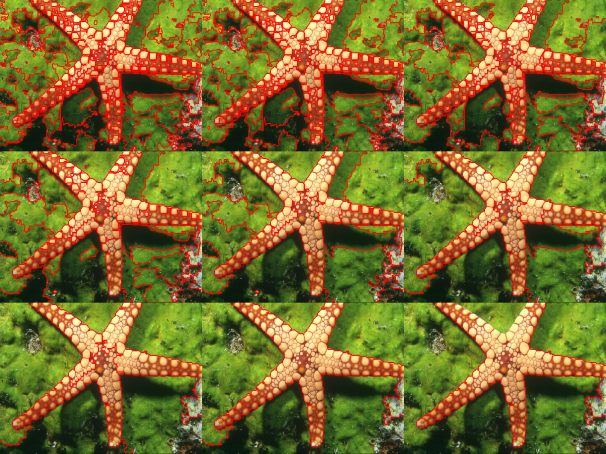
\includegraphics[width=3.5cm]{figures/图像BSDS12003的SRM结果线图.png}
    }
    \subfigure[SRM结果颜色图]
    {
        \label{Fig.sub.1}
        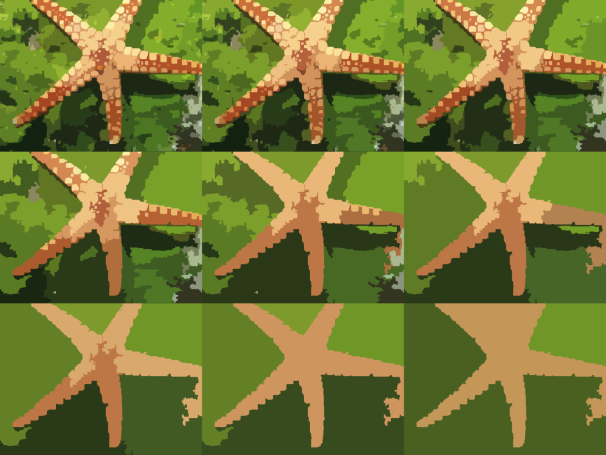
\includegraphics[width=3.5cm]{figures/图像BSDS12003的SRM结果颜色图.png}
    }
    \captionsetup{justification=centering}
    \caption{图像BSDS12003的SRM结果图 \\ Fig.\ref{SRM结果图1} Results Image BSDS12003 SRM are Illustrated}\label{SRM结果图1}
\end{figure}


\begin{figure}[H]
\centering
    \subfigure[SRM结果线图]
    {
        \label{Fig.sub.1}
        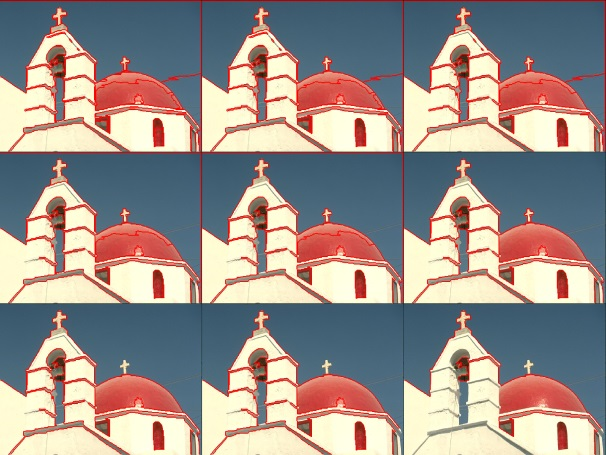
\includegraphics[width=3.5cm]{figures/图像BSDS118035的SRM结果线图.jpg}
    }
    \subfigure[SRM结果颜色图]
    {
        \label{Fig.sub.1}
        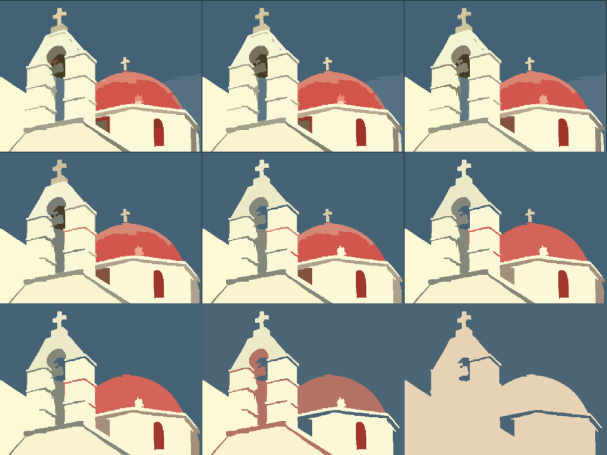
\includegraphics[width=3.5cm]{figures/图像BSDS118035的SRM结果颜色图.png}
    }
    \captionsetup{justification=centering}
    \caption{图像BSDS118035的SRM结果图 \\ Fig.\ref{SRM结果图2} Results Image BSDS118035 SRM are Illustrated}\label{SRM结果图2}
\end{figure}


\begin{figure}[H]
\centering
    \subfigure[SRM结果线图]
    {
        \label{Fig.sub.1}
        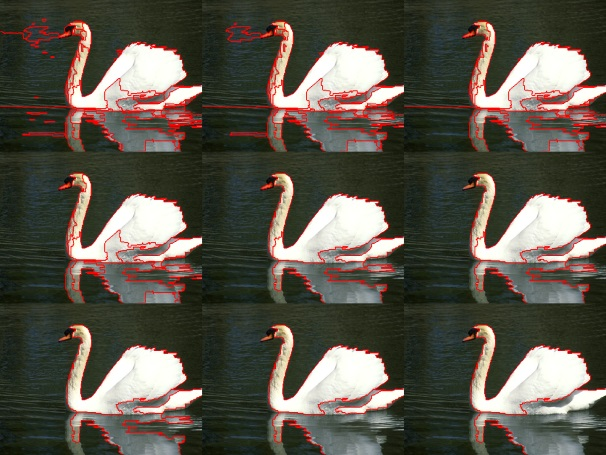
\includegraphics[width=3.5cm]{figures/图像BSDS8068的SRM结果线图.jpg}
    }
    \subfigure[SRM结果颜色图]
    {
        \label{Fig.sub.1}
        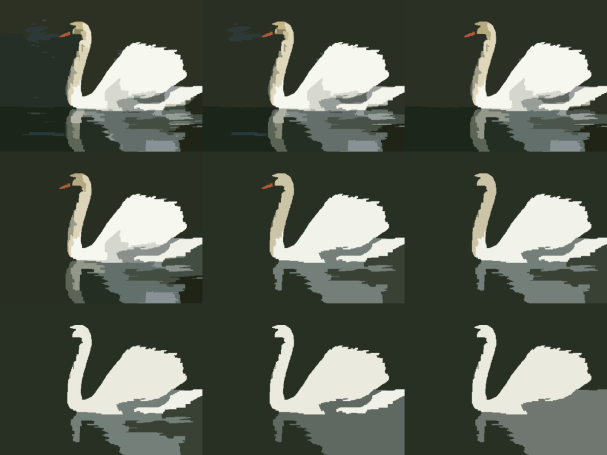
\includegraphics[width=3.5cm]{figures/图像BSDS8068的SRM结果颜色图.png}
    }
    \captionsetup{justification=centering}
    \caption{图像BSDS8068的SRM结果图 \\ Fig.\ref{SRM结果图3} Results Image BSDS8068 SRM are Illustrated}\label{SRM结果图3}
\end{figure}


\subsection{基于超像素表达的最优分割算法实验结果}

本部分实验使用基于超像素分割算法SLIC算法、聚类合并算法和区域邻接图RAG设计的面向目标提取的最优分割算法。

本部分实验的原始图像分为两部分:Berkeley图像数据库BSDS500和真实无人机航拍图像。针对上述两部分图像,调整必要参数,得到最优分割结果。由于谱聚类算法和RAG在本算法中的本质都是进行区域合并,所以本部分实验结果也分成两部分进行展示:包括谱聚类聚类区域合并结果和在谱聚类基础上的RAG区域合并结果。

\noindent{\textbf{(1) BSDS500数据库图像实验结果}}
\begin{figure}[H]
\centering
    \subfigure[谱聚类结果线图]
    {
        \label{Fig.sub.1}
        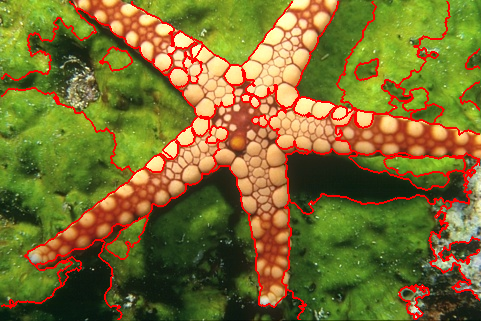
\includegraphics[width=3.5cm]{figures/图像BSDS12003的谱聚类结果线图.png}
    }
    \subfigure[谱聚类结果颜色图]
    {
        \label{Fig.sub.1}
        
\includegraphics[width=3.5cm]{figures/图像BSDS12003的谱聚类结果颜色图.png}
    }
    \subfigure[RAG结果线图]
    {
        \label{Fig.sub.1}
        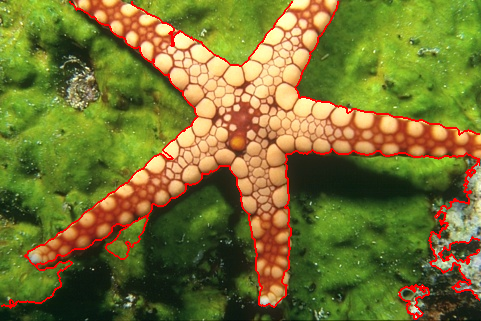
\includegraphics[width=3.5cm]{figures/图像BSDS12003的RAG结果线图.png}
    }
    \subfigure[RAG结果颜色图]
    {
        \label{Fig.sub.1}
        
\includegraphics[width=3.5cm]{figures/图像BSDS12003的RAG结果颜色图.png}
    }
    \captionsetup{justification=centering}
    \caption{图像BSDS12003的最优分割结果 \\ Fig.\ref{最优分割结果1} The image of BSDS12003 optimal segmentation result}\label{最优分割结果1}
\end{figure}

\begin{figure}[H]
\centering
    \subfigure[谱聚类结果线图]
    {
        \label{Fig.sub.1}
        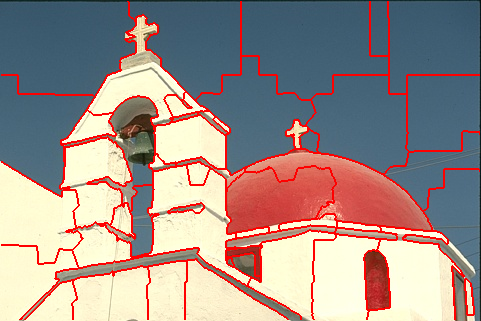
\includegraphics[width=3.5cm]{figures/图像BSDS118035的谱聚类结果线图.png}
    }
    \subfigure[谱聚类结果颜色图]
    {
        \label{Fig.sub.1}
        
\includegraphics[width=3.5cm]{figures/图像BSDS118035的谱聚类结果颜色图.png}
    }
    \subfigure[RAG结果线图]
    {
        \label{Fig.sub.1}
        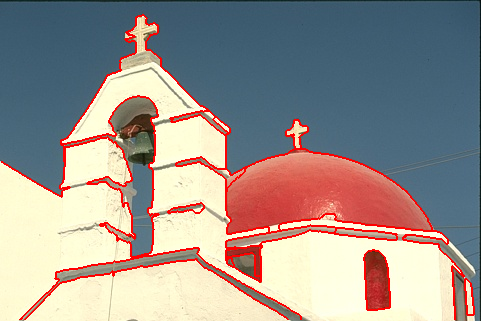
\includegraphics[width=3.5cm]{figures/图像BSDS118035的RAG结果线图.png}
    }
    \subfigure[RAG结果颜色图]
    {
        \label{Fig.sub.1}
        
\includegraphics[width=3.5cm]{figures/图像BSDS118035的RAG结果颜色图.png}
    }
    \captionsetup{justification=centering}
    \caption{图像BSDS118035的最优分割结果 \\ Fig.\ref{最优分割结果2} The image of BSDS118035 optimal segmentation result}\label{最优分割结果2}
\end{figure}


\begin{figure}[H]
\centering
    \subfigure[谱聚类结果线图]
    {
        \label{Fig.sub.1}
        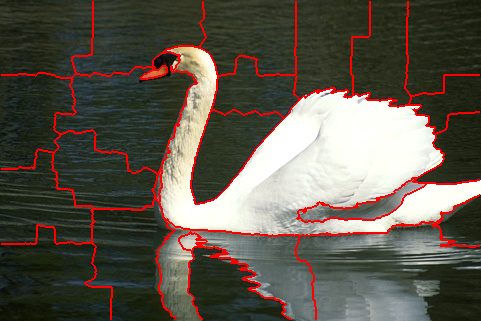
\includegraphics[width=3.5cm]{figures/图像BSDS8068的谱聚类结果线图.png}
    }
    \subfigure[谱聚类结果颜色图]
    {
        \label{Fig.sub.1}
        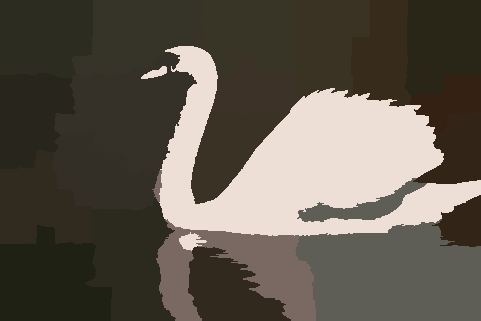
\includegraphics[width=3.5cm]{figures/图像BSDS8068的谱聚类结果颜色图.png}
    }
    \subfigure[RAG结果线图]
    {
        \label{Fig.sub.1}
        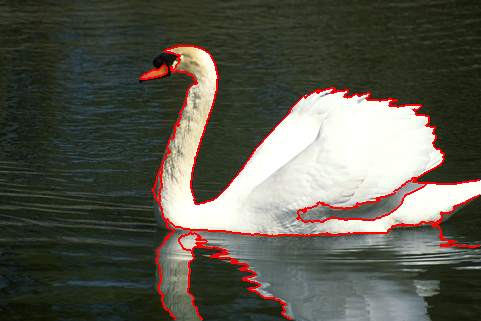
\includegraphics[width=3.5cm]{figures/图像BSDS8068的RAG结果线图.png}
    }
    \subfigure[RAG结果颜色图]
    {
        \label{Fig.sub.1}
        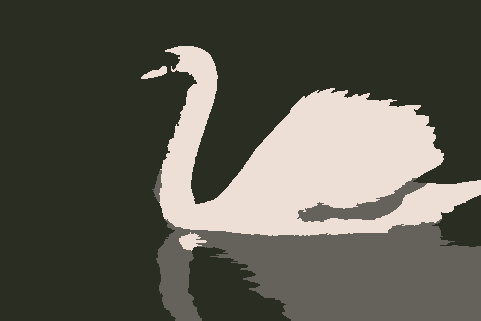
\includegraphics[width=3.5cm]{figures/图像BSDS8068的RAG结果颜色图.png}
    }
    \captionsetup{justification=centering}
    \caption{图像BSDS8068的最优分割结果 \\ Fig.\ref{最优分割结果3} The image of BSDS8068 optimal segmentation result}\label{最优分割结果3}
\end{figure}

\noindent{\textbf{(2) 无人机航拍图像实验结果}}


\begin{figure}[H]
\centering
    \subfigure[谱聚类结果线图]
    {
        \label{Fig.sub.1}
        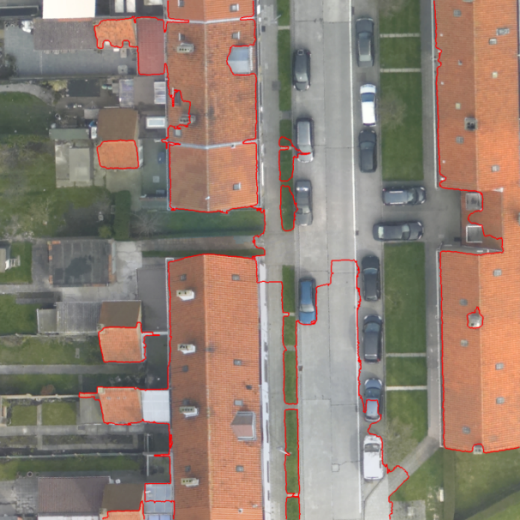
\includegraphics[width=3.2cm]{figures/无人机航拍图像1RAG结果线图.png}
    }
    \subfigure[谱聚类结果颜色图]
    {
        \label{Fig.sub.1}
        
\includegraphics[width=3.2cm]{figures/无人机航拍图像1RAG结果颜色图.png}
    }
    \subfigure[RAG结果线图]
    {
        \label{Fig.sub.1}
        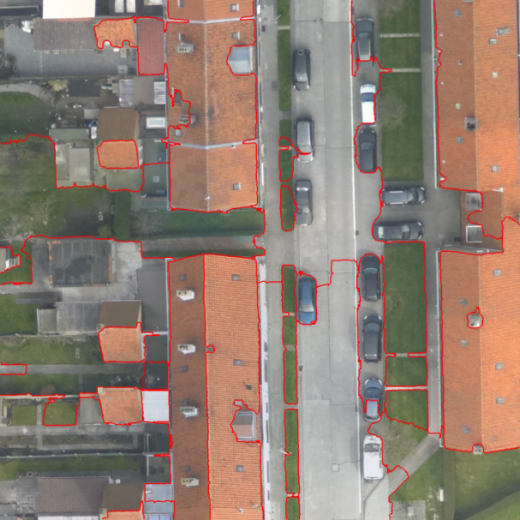
\includegraphics[width=3.2cm]{figures/无人机航拍图像1谱聚类结果线图.png}
    }
    \subfigure[RAG结果颜色图]
    {
        \label{Fig.sub.1}
        
\includegraphics[width=3.2cm]{figures/无人机航拍图像1谱聚类结果颜色图.png}
    }
    \captionsetup{justification=centering}
    \caption{无人机航拍图像1的最优分割结果 \\ Fig.\ref{无人机最优分割结果1} 1 the optimal segmentation result unmanned aerial images}\label{无人机最优分割结果1}
\end{figure}


\begin{figure}[H]
\centering
    \subfigure[谱聚类结果线图]
    {
        \label{Fig.sub.1}
        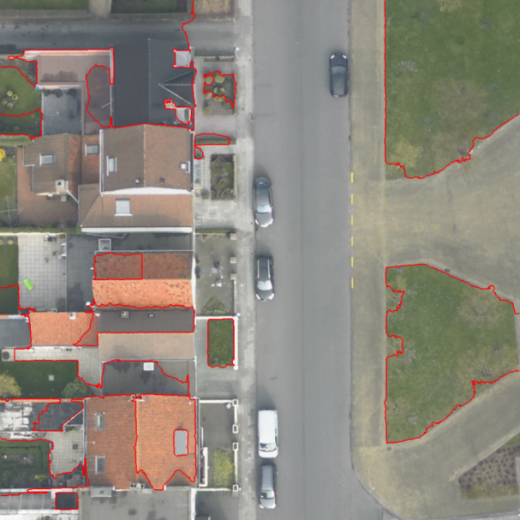
\includegraphics[width=3.2cm]{figures/无人机航拍图像2RAG结果线图.png}
    }
    \subfigure[谱聚类结果颜色图]
    {
        \label{Fig.sub.1}
        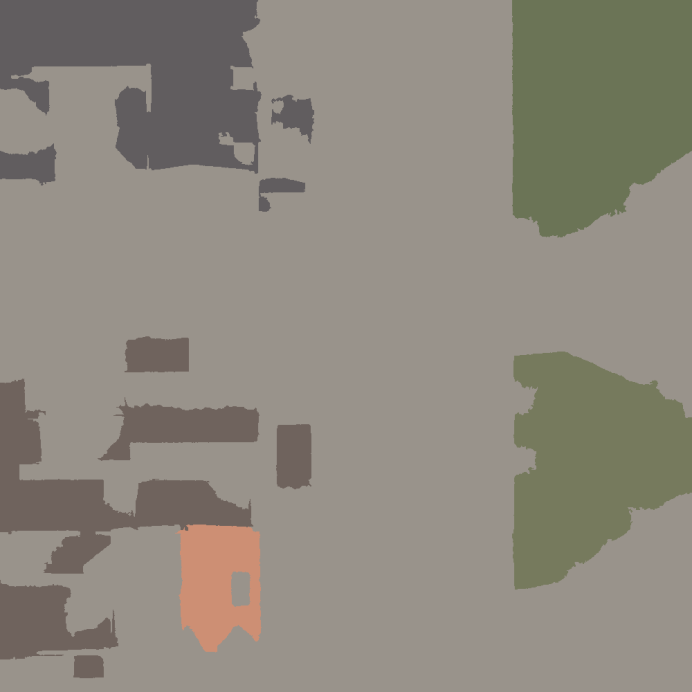
\includegraphics[width=3.2cm]{figures/无人机航拍图像2RAG结果颜色图.png}
    }
    \subfigure[RAG结果线图]
    {
        \label{Fig.sub.1}
        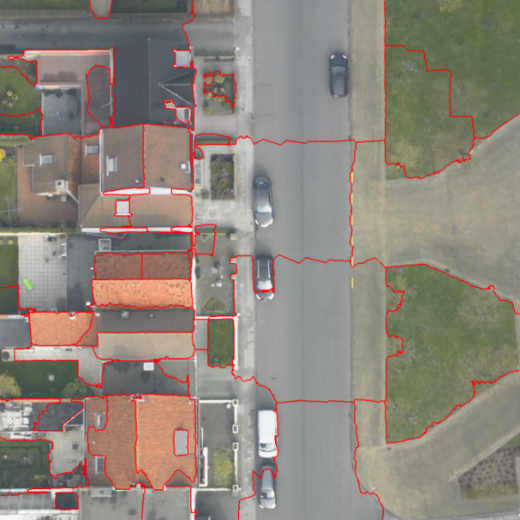
\includegraphics[width=3.2cm]{figures/无人机航拍图像2谱聚类结果线图.png}
    }
    \subfigure[RAG结果颜色图]
    {
        \label{Fig.sub.1}
        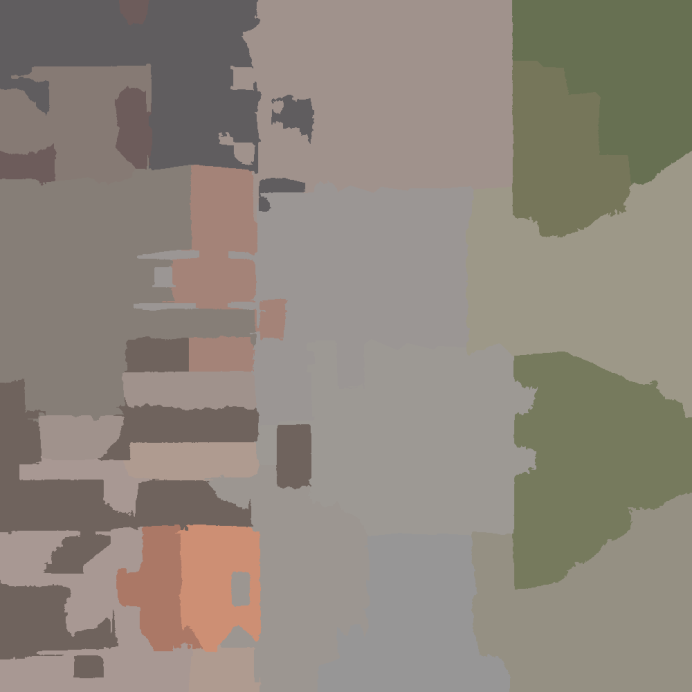
\includegraphics[width=3.2cm]{figures/无人机航拍图像2谱聚类结果颜色图.png}
    }
    \captionsetup{justification=centering}
    \caption{无人机航拍图像2的最优分割结果\\ Fig.\ref{无人机最优分割结果2} 2 the optimal segmentation result unmanned aerial images}\label{无人机最优分割结果2}
\end{figure}


\begin{figure}[H]
\centering
    \subfigure[谱聚类结果线图]
    {
        \label{Fig.sub.1}
        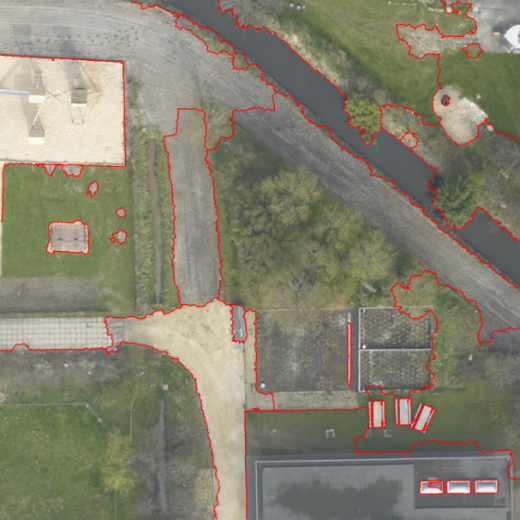
\includegraphics[width=3.2cm]{figures/无人机航拍图像3RAG结果线图.png}
    }
    \subfigure[谱聚类结果颜色图]
    {
        \label{Fig.sub.1}
        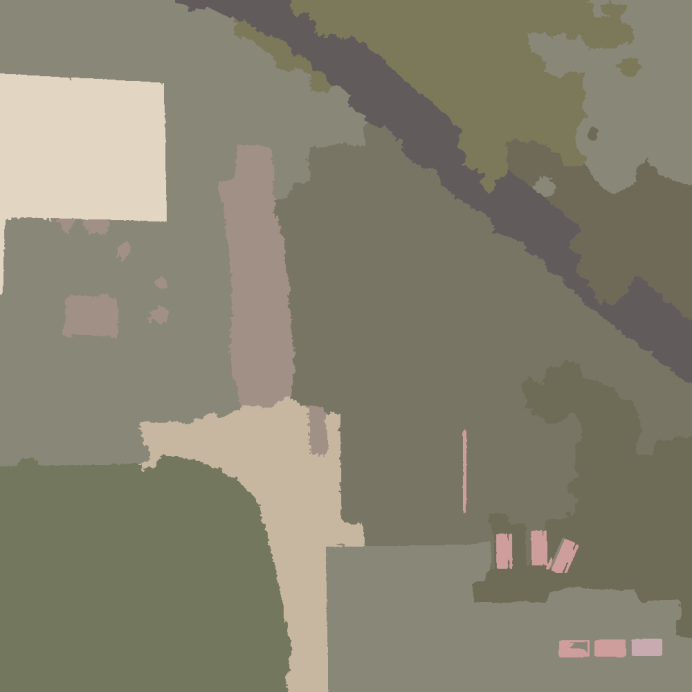
\includegraphics[width=3.2cm]{figures/无人机航拍图像3RAG结果颜色图.png}
    }
    \subfigure[RAG结果线图]
    {
        \label{Fig.sub.1}
        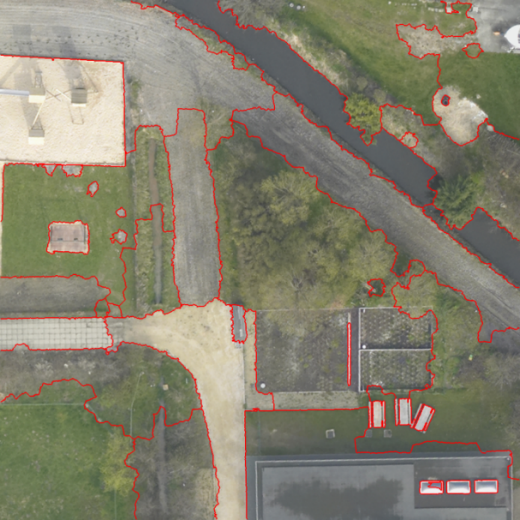
\includegraphics[width=3.2cm]{figures/无人机航拍图像3谱聚类结果线图.png}
    }
    \subfigure[RAG结果颜色图]
    {
        \label{Fig.sub.1}
        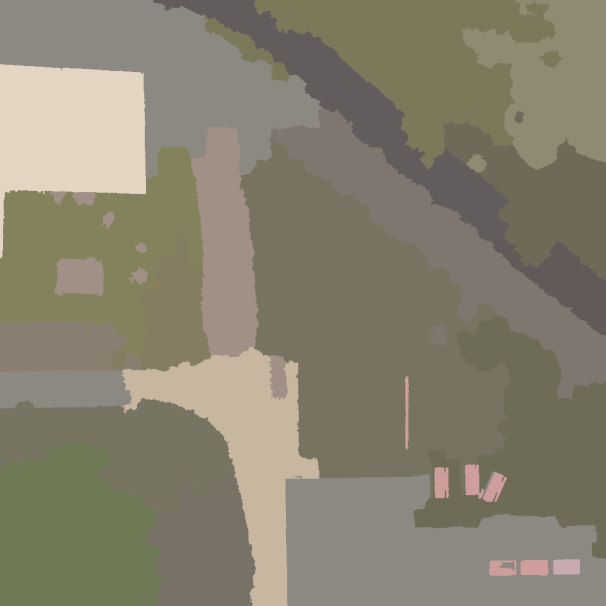
\includegraphics[width=3.2cm]{figures/无人机航拍图像3谱聚类结果颜色图.png}
    }
    \captionsetup{justification=centering}
    \caption{无人机航拍图像3的最优分割结果\\ Fig.\ref{无人机最优分割结果3} 3 the optimal segmentation result unmanned aerial images}\label{无人机最优分割结果3}
\end{figure}



\subsection{实验结果分析}

由图\ref{SRM结果图1}和\ref{SRM结果图2}可以清楚的看出,$Q$取值不同,分割结果不同,$Q$值越小,分割结果中聚类数量越少,当$Q$取值合理的时候,能将前景目标与背景分离出来。

本部分实验使用两部分数据进行实验,一部分是Berkeley图像数据库,另一部分是真实的无人机航拍图像。
由图\ref{最优分割结果1}、\ref{最优分割结果2}和\ref{最优分割结果3}可以清楚的看出,经过谱聚类和RAG两次区域合并,能将大部分的超像素块正确进行合并,并将前景目标和背景进行分离。但是,同时由图\ref{无人机最优分割结果1}、\ref{无人机最优分割结果2}和\ref{无人机最优分割结果3}能够看出,基于超像素的最优分割算法在场景较为复杂的时候分割效果不够理想,许多超像素块被错误合并。
